% !TEX root = BA-Bauer.tex

\subsection{Platinendesign} \label{sec:PCB-Design}
Das Design der Platine spielt eine wichtige Rolle in der Entwicklung des Gerätes, denn es müssen alle 78\,Komonenten auf ihr Platz finden, sie muss elektrisch und logisch sinnvoll aufgebaut sein und gleichzeitig kompakte Maße haben damit das Endprodukt handlich ist. Zudem kommen einige technische Anforderung von Bauteilen wie die Platzierung der Stützkondensatoren des MCUs, die möglichst nah an ihm platziert werden müssen, hinzu. Außerdem muss der SD-Karten-Steckplatz im nachhinein für den Benutzer zugänglich sein, der Benutzer muss die Taster betätigen, die LEDs leuchten, den LCD sehen können und in der Lage dazu sein die DMX- und das USB-Kabel in die entsprechenden Buchsen zu stecken.
\begin{figure}[h]
	\centering
	\begin{minipage}[t]{0.47\linewidth}
		\centering
		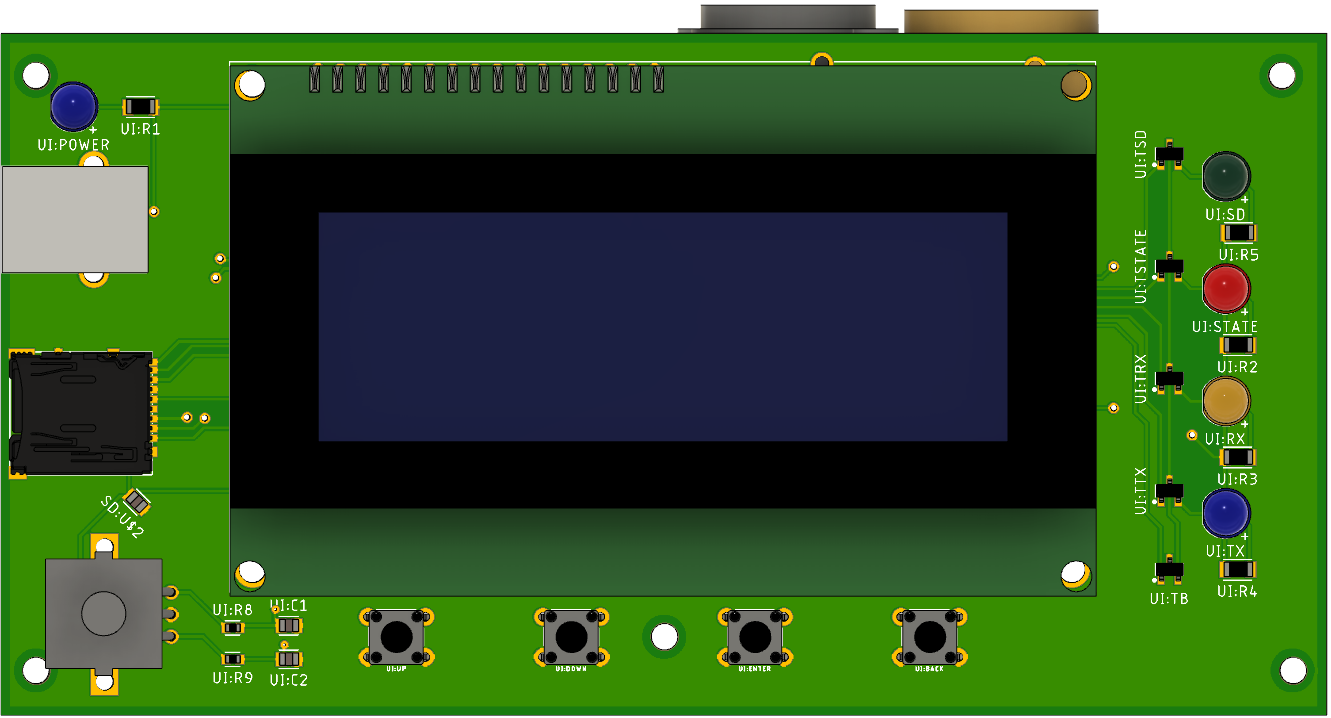
\includegraphics[width=\linewidth]{PCB_top}
		\caption{Platinenvorderseite}
		\label{fig:PCB-top}
	\end{minipage}
	\hfil
	\begin{minipage}[t]{0.47\linewidth}
		\centering
		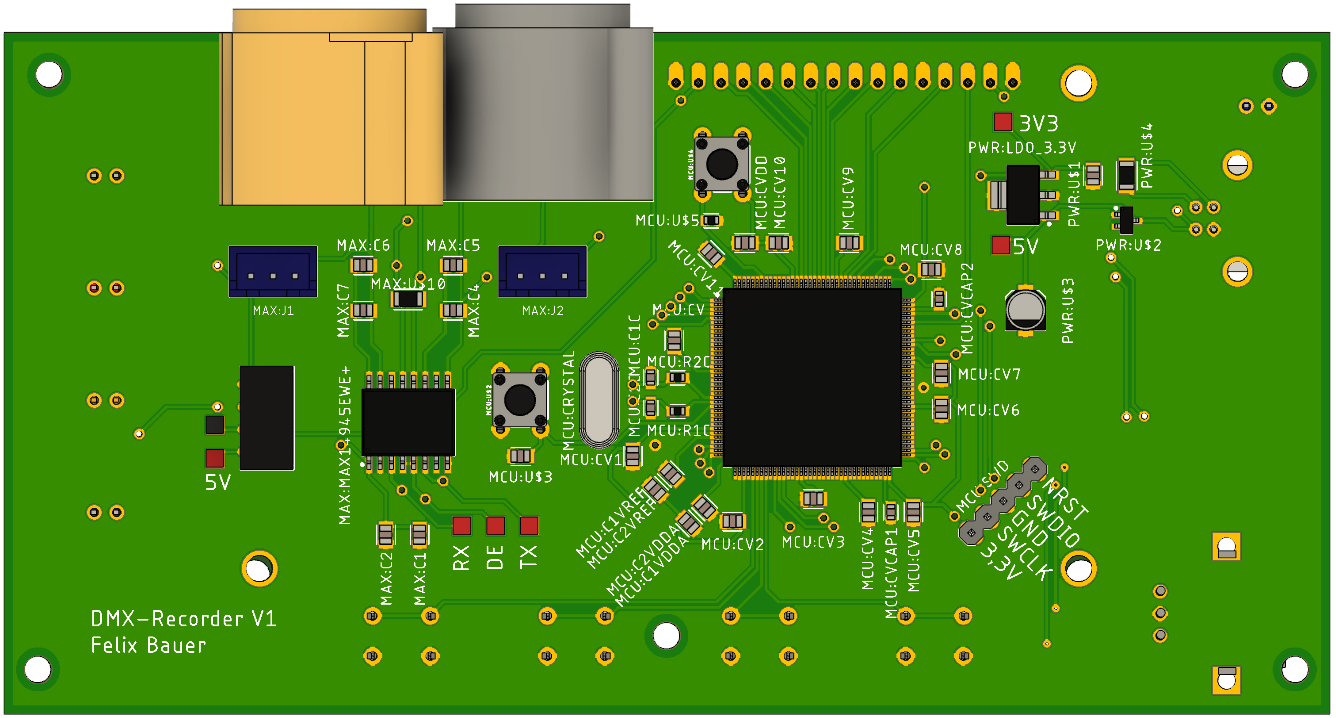
\includegraphics[width=\linewidth]{PCB_bottom}
		\caption{Platinenrückseite}
		\label{fig:PCB-bottom}
	\end{minipage}
\end{figure}\\
Abbildung \ref{fig:PCB-top} und \ref{fig:PCB-bottom} zeigen das Layout der Platine als virtuelles dreidimensionales Modell. 
%Die Platinenentwicklungssoftware \textit{EAGLE}\footnote{https://www.autodesk.de/products/eagle/overview} der Firma \textit{Autodesk} kann in Verbindung mit der ebenfalls von \textit{Autodesk} entwickelten 3D-CAD-Software \textit{Fusion 360}\footnote{https://www.autodesk.de/products/fusion-360/overview} ein virtuelles Modell der Platine automatisiert erstellen. Dieses kann dafür genutzt werden um Kollisionen von einzelnen Komponenten vorab abzuwenden und erleichtert das Konstruieren eines Gehäuses. Zudem gibt es die Möglichkeit die Dimnsionierung der Platine in \textit{Fusion 360} festzulegen und an \textit{EAGLE} zu übergeben. Damit eine möglichst genaue dreidmensionale Abbildung möglich ist, ist es notwendig die einzelnen Komponenten als 3D-Modell zu erstellen. \textit{EAGLE} bietet einen internen Modell-Generator zum generieren von üblichen Komponentenformen. Einige Hersteller bieten außerdem 3D-Modelle als Download an. 
Auf der Platine werden zwei Arten von Komponenten verbaut. Zum einen sogenannte \textit{surface-mount-technology}-Komponenten (SMT-Komponenten), zum anderen \textit{through-hole technology}-Komponenten (THT-Komponenten). SMT-Komponenten werden direkt auf die Oberfläche der Platine gelötet, was keine Notwendigkeit von Löchern in der Platine erfordert. Durch die Oberflächenmotage befindet sich das Bauteil auch auf der selben Seite wie die dazugehörige Lötstelle. Für THT-Komponenten werden Löcher in der Platine benötigt, da die Pins der Komponenten im 90 Grad Winkel zur Oberfläche der Platine gerichtet sind. Diese können unter Umständen nur auf der gegenüberliegenden Seite der Platine verlötet werden. Eine LED zum Beispiel, die bündig mit der Platine verlötet werden soll, kann nur auf der gegenüberliegenden Seite der Platine verlötet werden, da die LED selbst ihre eigenen Pins verdeckt. Damit alle Komponenten frei auf der Platine platziert werden können, wird eine zweiseitige Platine entworfen. Diese besitzt auf der Vorder- und Rückseite eine Kupferschicht, welche mithilfe von sogenannten \textit{Vias}\footnote{Durchkontaktierte Löcher in der Platine} verbunden werden können.
\begin{figure}[h]
	\begin{center}
		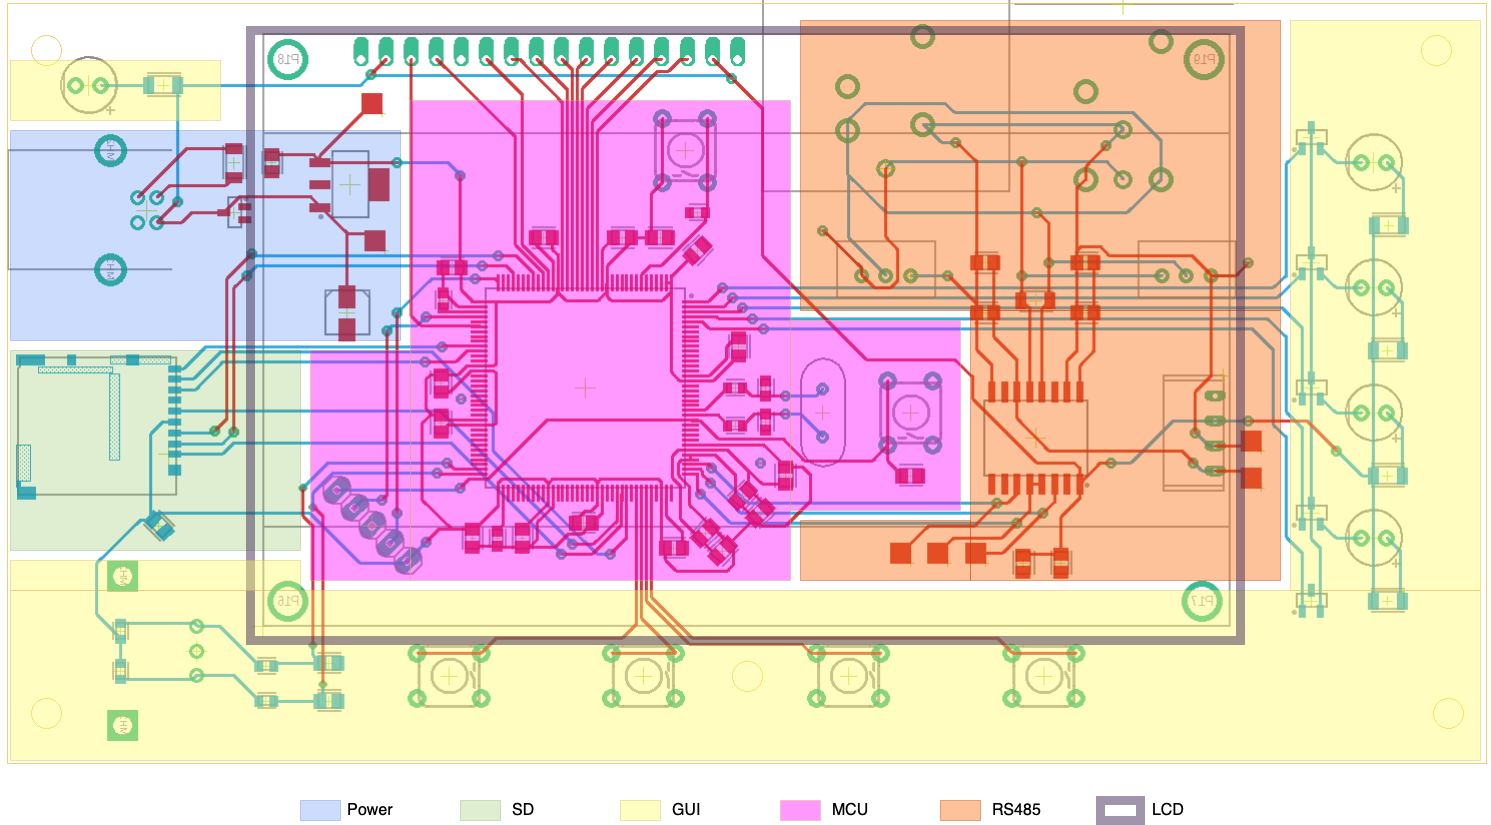
\includegraphics[width=\linewidth]{PCB-Design_mark}
		\caption{Platinenlayout-Aufteilung}
		\label{fig:PCB-Layout}
	\end{center}
\end{figure}
Abbildung \ref{fig:PCB-Layout} zeigt die generelle Aufteilung der Platine. Diese Aufteilung vereinfacht die mögliche Fehlersuche und trägt dazu bei die Leiterbahnlängen zu verkürzen. Alle blau gefärbten $Pads$\footnote{In der Regel rechteckige Lötstellen (freigelegte Kupferflächen) zum verlöten von SMT-Komponenten} und Leiterbahnen befinden sich auf der Vorderseite, alle rot eingefärbten auf der Rückseite der Platine. Die freien Flächen zwischen den Leiterbahnen auf der Ober- und Unterseite sind mit dem 0\,V Potential verbunden. Die grünen Bohrungen sind $Vias$ und durchkontaktiert Bohrungen für die THT-Komponenten.
Der Formfaktor der Platine wird im wesentlichen von dem LCD-Modul vorgegeben, da es bei weitem das größte Bauteil darstellt. Neben dem LCD-Modul muss außerdem Platz für den Encoder, die Taster und LEDs vorhanden und für den Benutzer sichtbar und verwendbar sein. Aus diesem Grund werden das LCD-Modul, die Taster, der Encoder und die LEDs auf der Vorderseite der Platine platziert. Im Zentrum befindet sich das LCD-Modul. Unterhalb des Moduls befinden sich die Taster, rechts davon die LEDs. Die LED, die den Zustand der Spannngsversorgung anzeigt befindet sich oben links um eine Verwechslungen mit der zweiten blauen LED zu verhindern. Der SD-Kartensteckplatz, grün markiert, findet am linken Rand unterhalb der USB-Buchse und Schaltung der Spannungsversorgung, blau markiert, der Platine Platz. Der MCU bildet das Herzstück der Schaltung und befindet sich deswegen  in der Mitte der Platine. Laut Hersteller sollen die Stützkondensatoren möglichst nah am MCU plaziert werden, damit die Induktivität der Leiterbahnen den hohen Stromfluss aus den Kondensatoren heraus nicht beeinträchtigt. \textbf{Erklärung / Quelle} Kritische an den MCU angeschlossene Komponenten sind unter anderem der SD-Kartenslot, der Quartz und der RS485-Treiberchip. Um möglichst wenig Störungen auf die Leiterbahnen einwirken zu lassen sind diese möglichst kurz. Die XLR-Buchsen für die ein- und ausgehenden DMX-Daten befinden sich am oberen Rand der Rückseite der Platine. Sie und die Schaltung des Treiberchips, rot markiert, liegen nah beieinander um auch hier das Störungspotential durch lange Leiterbahnen möglichst gering zu halten.